\section{Аналитические раздел}


\subsection{Реализация алгоритма}

\begin{lstlisting}
	GENERATE (UNIFORM(1, 1.0, 10.0))
	IN QUEUE RequestQueue
	SEIZE Service
	DEPART RequestQueue
	ADVANCE (POISSON(1, 1))
	RELEASE Service
	TRANSFER 0.0,OUT,IN 
	OUT TERMINATE 0
	
	GENERATE 100000
	TERMINATE 1
	START 1	
\end{lstlisting}

\section{Результаты работы}

В результате разработана программа, позволяющая промоделировать
систему событийным принципом с указанием параметров.

На рисунке \ref{fig:r2} редставлен результат работы программы при $a=1.0$, $b = 10.0$, $\lambda=1$. Максимальный размер очереди --- 19.

\begin{figure}[ht!]
	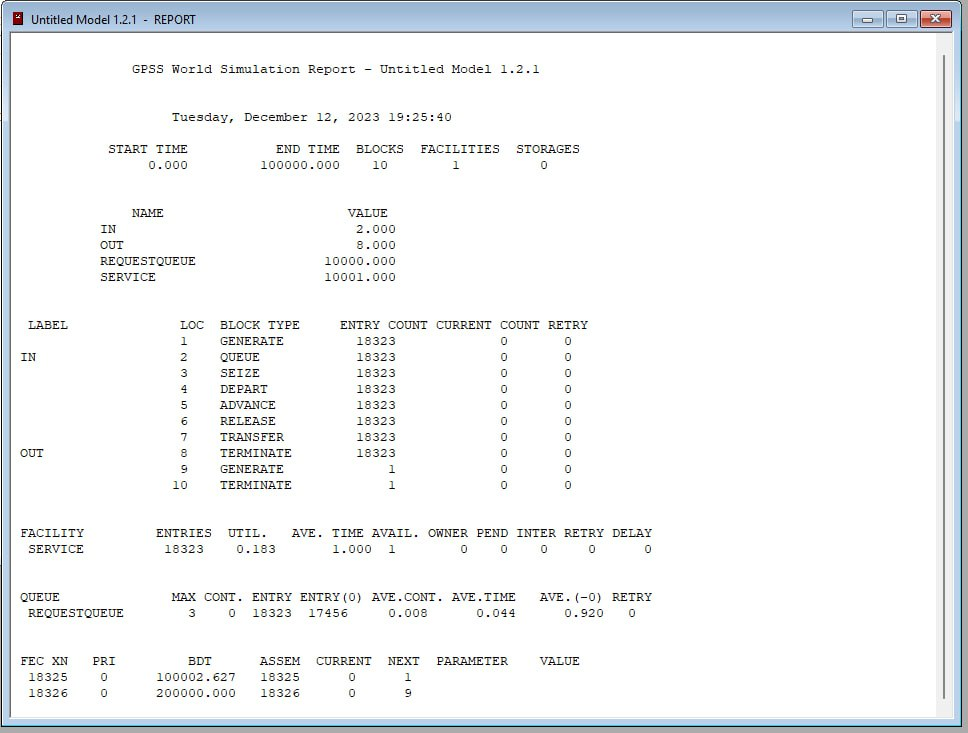
\includegraphics[width=0.75\linewidth]{assets/images/res.png}
	\caption{Результаты работы программы}
	\label{fig:r2}
\end{figure}